%% hf: enable header and footer.
\documentclass[
twocolumn,
% hf,
]{ceurart}

% One can fix some overfills
% \sloppy

% This was used to mitigate some warnings
\usepackage[T1]{fontenc}
\usepackage{lmodern}

\begin{document}

% Rights management information. CC-BY is the default license.
\copyrightyear{2024}
\copyrightclause{Copyright for this paper by its authors.
  Use permitted under Creative Commons License Attribution 4.0
  International (CC BY 4.0).}

\conference{BPM 2024: Demos and Resources, September 01-06, 2024, Krakow, PL}

\title{BPMN Analyzer 2.0: Instantaneous, Comprehensible, and Fixable Anomaly Detection for Realistic BPMN Models}

\author[1]{Tim Kräuter}
[email=tkra@hvl.no]
\author[1]{Patrick Stünkel}
[email=past@hvl.no] % patrick.stuenkel@hvl.no
\author[1]{Adrian Rutle}
[email=aru@hvl.no]
\author[1]{Yngve Lamo}
[email=yla@hvl.no]
\author[2,1]{Harald König}
[email=harald.koenig@fhdw.de]
\address[1]{Western Norway University of Applied Sciences, Bergen, Norway}
\address[2]{FHDW Hannover, Germany}

\begin{abstract}
  The tool is available online.
\end{abstract}

\begin{keywords}
BPM,
Verification,
Soundness,
Safeness
\end{keywords}

\maketitle

% Details can be found here: https://bpm2024.agh.edu.pl/call-for-demos-and-resources/

\section{Introduction}
The tool is available online\footnote{\url{https://timkraeuter.com/bpmn-analyzer-js/}} alongside a video demonstration\footnote{\url{https://www.youtube.com/watch?v=MxXbNUl6IjE}}.
% Why is it significant for the BPM field?

\begin{figure}[ht]
	\centering
	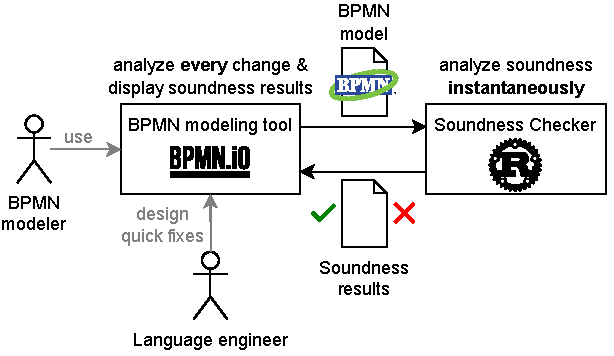
\includegraphics[width=\linewidth]{images/overview}
	\caption{Overview of the tool}
	\label{fig:overview}
\end{figure}

\section{Innovations?} % Main tool description and showing the innovations
Three main innovations of the tool:
% Instantaneous
% Comprehensible
% Fixable

\section{Maturity of the tool}
% Scalability tests (instantaneous)
Improves upon our previous BPMN Analyzer tool~\cite{krauterFormalizationAnalysisBPMN2023}.
% bpmn.io forum link/mention: https://forum.bpmn.io/t/automatic-bpmn-control-flow-analysis-and-resolution/11150


% \begin{acknowledgments}
% Thanks to the anonymous reviewers for their valuable feedback.
% \end{acknowledgments}

\section{Related work?}
% Could cite my other extended version and put that on arxiv.

\section{Conclusion \& future work}

\bibliography{bib}

% If your work has an appendix, this is the place to put it.
% \appendix

\end{document}
